\subsection{系统调用}

首先实现一个提供加法服务的系统调用\texttt{syscall\_0}。

\begin{figure}[H]
    \centering
    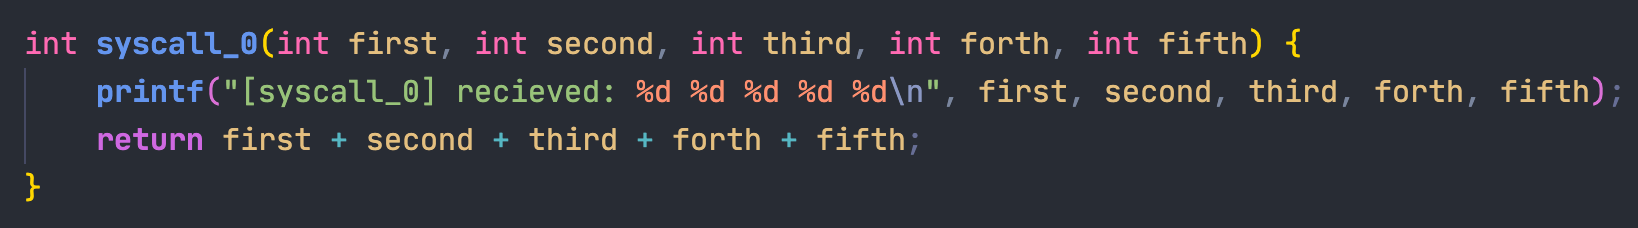
\includegraphics[width=0.6\textwidth]{figures/zeroSyscall.png}
    \label{zeroSyscall}
\end{figure}

它可以返回参数的和,并且将它们打印到屏幕上。

根据文档实现了处理中断的函数\texttt{asm\_system\_call()}。
并实现了系统调用类\texttt{SystemService}。

然后编写如下使用了系统调用的线程。

\begin{figure}[H]
    \centering
    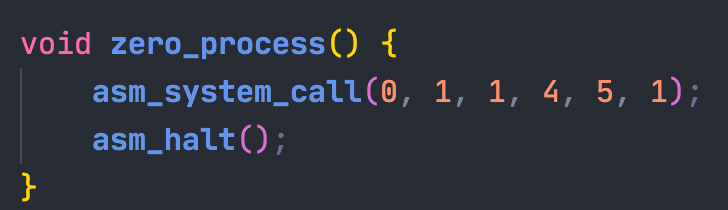
\includegraphics[width=0.6\textwidth]{figures/zero.png}
    \label{zero}
\end{figure}

观察实验结果,

\begin{figure}[H]
    \centering
    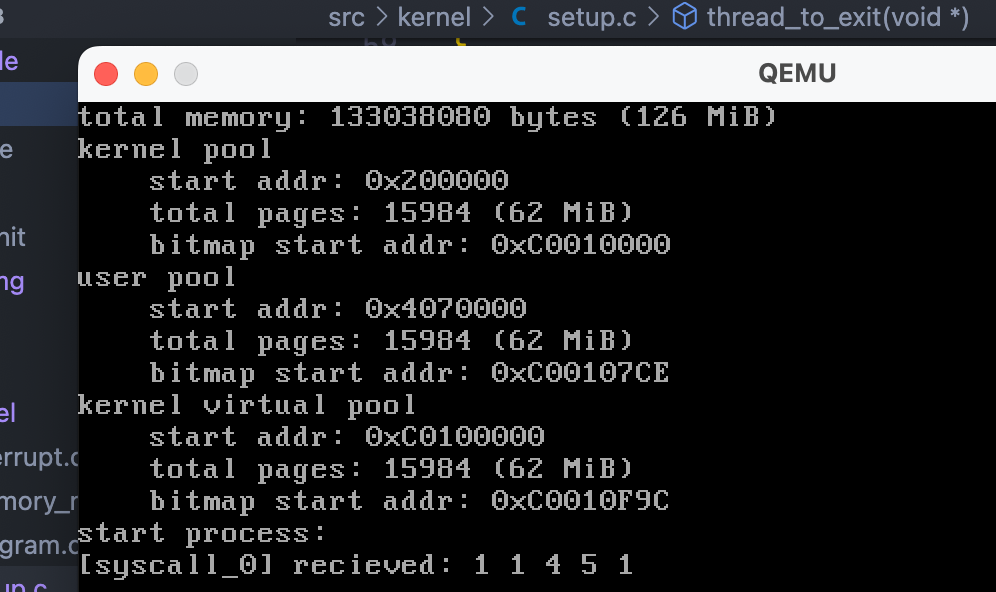
\includegraphics[width=0.6\textwidth]{figures/zeroRes.png}
    \label{zeroRes}
\end{figure}

可以发现系统调用得到了正确调用。

\subsection{\texttt{fork()}的设计与实现}

在\texttt{fork()}之前,我们先需要实现进程以及用户地址空间,
具体实现步骤大体参照文档完成。

为了实现进程,需要将内核的相对地址提升到\texttt{0x0c000000}之后,
并且提前开启分页机制。之后需要对TSS进行定义和实现。准备工作完成后,
可以开始实现进程。

用户级进程拥有自己的地址池,所以需要在PCB中加上用户地址池成员以及对应的页表地址。
所以在初始化进程时,需要进行PCB分配、页表分配以及用户地址池初始化三步。

而进程的调度需要在已经实现的线程调度上增加更换内存页目录表以及更换用户栈两个过程。
具体实现根据文档的指引完成,此处不在赘述。

为了验证结果,将调用\texttt{syscall\_0}的线程改为进程。

\begin{figure}[H]
    \centering
    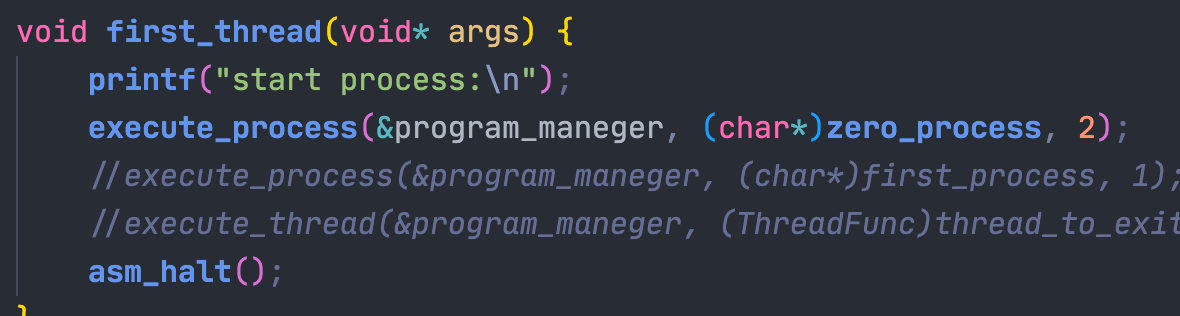
\includegraphics[width=0.6\textwidth]{figures/process.png}
    \label{process}
\end{figure}

观察实验结果,

\begin{figure}[H]
    \centering
    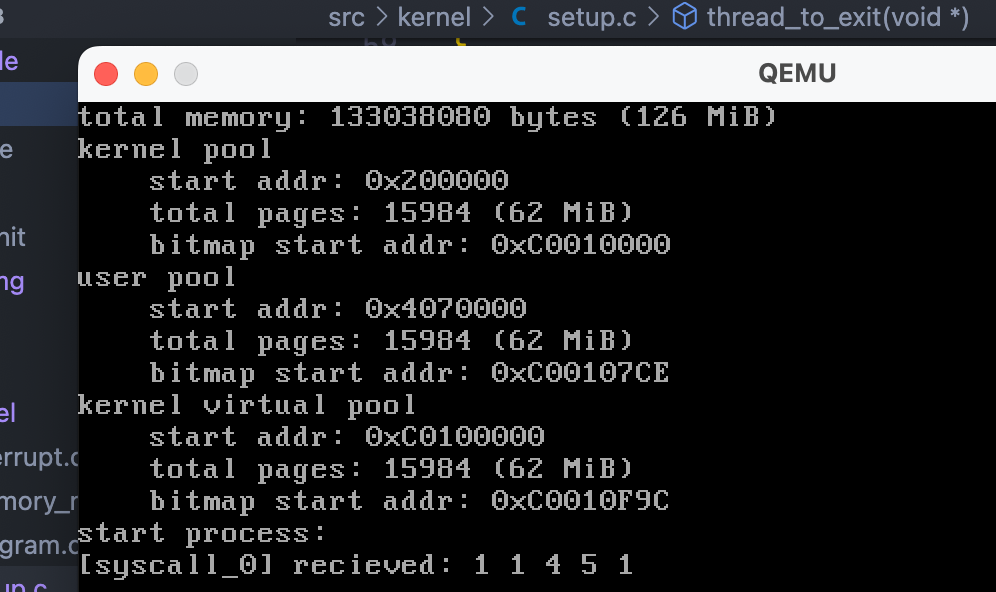
\includegraphics[width=0.6\textwidth]{figures/zeroRes.png}
    \label{zeroRes1}
\end{figure}

即使变成了进程,我们的系统调用依然可以正确运行。

那么就可以接着实现\texttt{fork()}了,它的作用是复制调用它的进程,如果他是
上级进程,则返回复制生成的新进程的pid,如果是下级进程则返回0。根据文档
依次实现新进程的创建、PCB的复制、用户栈的复制以及最为关键的返回地址的复制,于是
完成了这个系统调用。

为了验证结果,构造以下进程。

\begin{figure}[H]
    \centering
    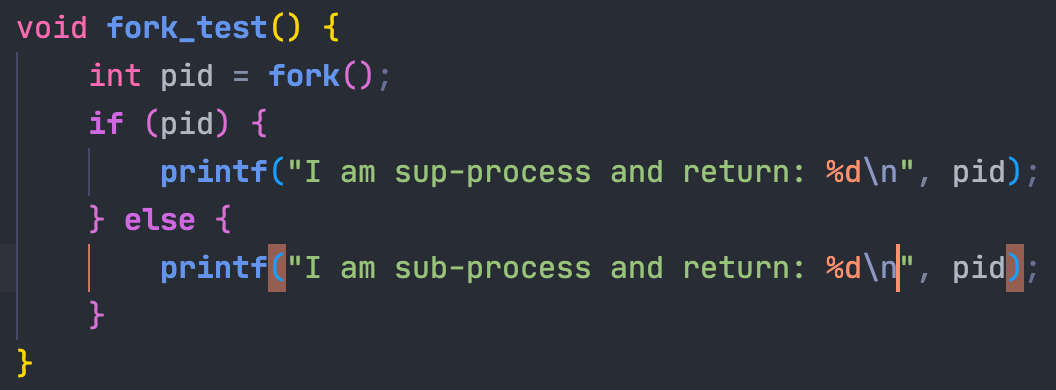
\includegraphics[width=0.6\textwidth]{figures/forkTest.png}
    \label{forkTest}
\end{figure}

观察实验结果,

\begin{figure}[H]
    \centering
    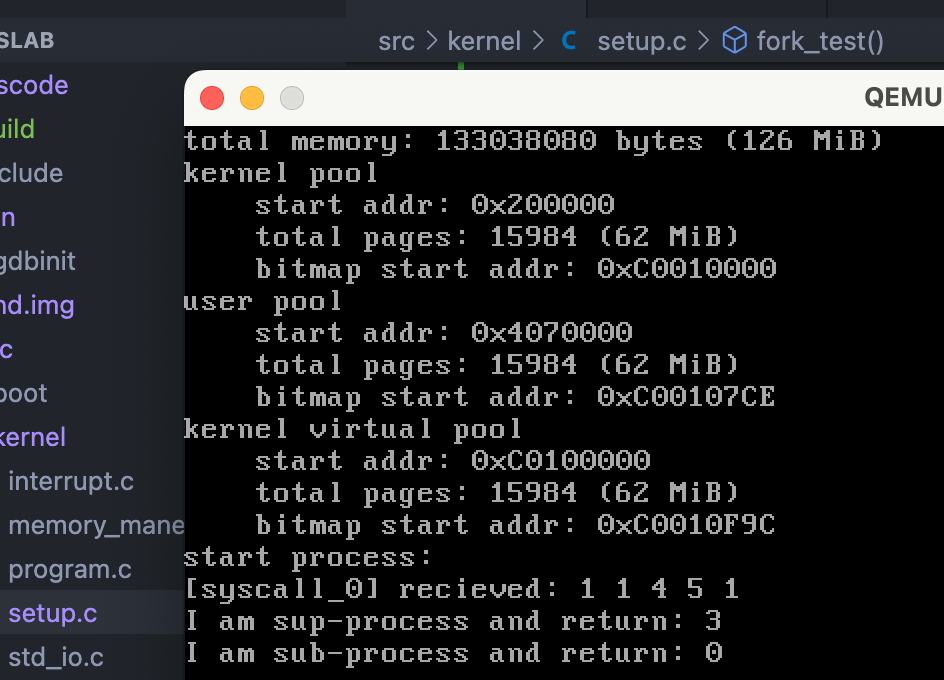
\includegraphics[width=0.6\textwidth]{figures/forkRes.png}
    \label{forkRes}
\end{figure}

可以看到\texttt{fork()}在上下级两个进程各返回了一次,且上级进程返回的是
下级进程的pid。

\subsection{\texttt{wait()}与\texttt{exit()}的设计与实现}

\texttt{exit()}的实现较为简单,只需要按照文档完成“将PCB状态置为\texttt{DEAD}并放入返回值”,
“释放进程的用户地址空间(如果有)”以及“立即进行进程调度”三个步骤即可。

而\texttt{wait()}的作用是令上级进程等待其下级进程执行完毕并回收PCB、获取返回值。
实现过程参照课程文档:使用这个系统调用的进程会遍历其下级进程,如果不存在下级进程则返回-1,
如果存在且可以回收则返回其返回值,如果存在但不可回收则进程阻塞直到下级进程可以回收。

实现后构造以下进程验证:

\begin{figure}[H]
    \centering
    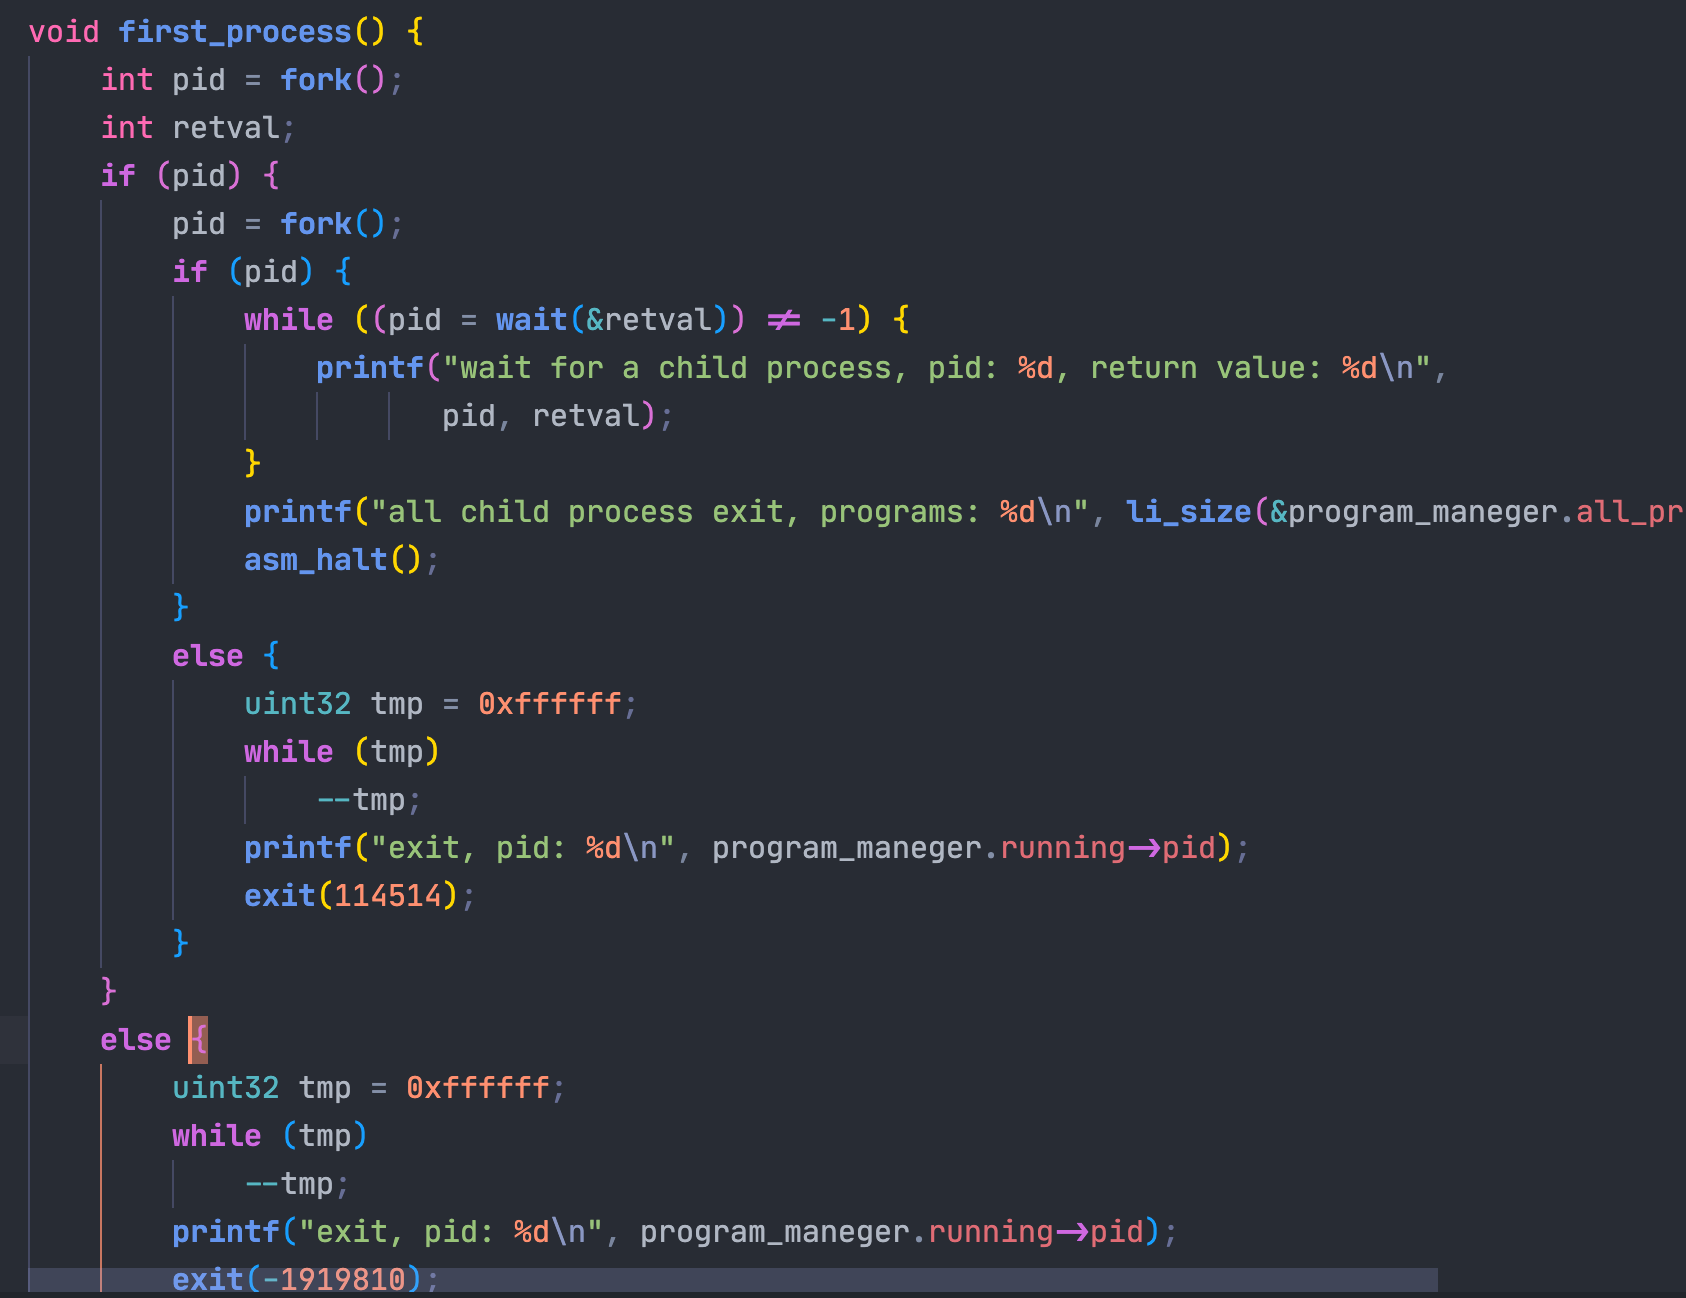
\includegraphics[width=0.6\textwidth]{figures/firstText.png}
    \label{firstText}
\end{figure}

可以看到进程中会使用\texttt{fork()}创造为三级进程,层层等待其下级进程的返回。
观察结果:

\begin{figure}[H]
    \centering
    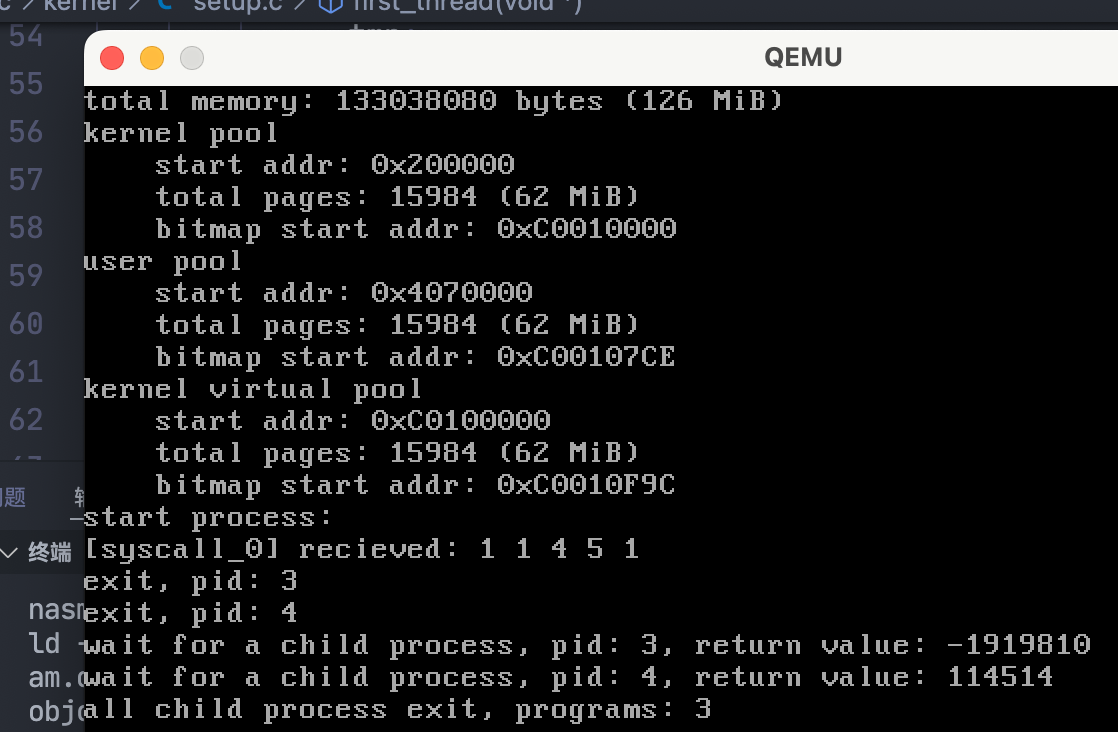
\includegraphics[width=0.6\textwidth]{figures/firstRes.png}
    \label{firstRes}
\end{figure}

可以观察到三级进程全部成功阻塞并返回。至此代码复现任务完成。